\chapter{Estimation of Rider Torque}

Given  the steer rate (\ensuremath{\dot{\delta}}) and acceleration(\ensuremath{\ddot{\delta}}), moment of inertia (\ensuremath{I_H}), motor damping  (\ensuremath{b_m}) and the torque applied by the handlebar motor (\ensuremath{T_{PDH}}) the equation of motion of the upper handlebar assembly can be formed (see Fig. \ref{fig:free_handle}) and solved for the uknown rider input torque (\ensuremath{T_H}).

\begin{equation}
    T_{H}= \ddot{\delta}I_H+\dot{\delta}b_{m} -T_{PDH} 
    \label{eq:torque_rider}
\end{equation}
\begin{figure}[h]
    \centering 
    \captionsetup{justification=centering,margin=2cm}

    \captionsetup{justification=centering,margin=2cm}
    \includegraphics[scale=0.9]{images/free_handle.png}
    \caption[Short title]{Free body diagram of the upper handlebar assembly. }
    \label{fig:free_handle}
\end{figure}

\section{Steer rate and acceleration} \label{sec:rateAccel}
Since only the steering angle is directly measurable, a way needs to be found that produces accurate estimations of steer rate and steer acceleration. Simple numerical differencing techniques proved ineffective as noise effects were magnified resulting in completed corrupted second derivatives, even after filtering the original signal to a cutoff frequency of 10 Hz. 

To combat this problem a piecewise cubic interpolation technique using the cubic spline function was used. The principle of this method is simple. Third order polynomilas are fitted   between the datapoints. This results in a signal that is identical to the original but instead of discrete points, it is represented by the union of polynomial functions. After this point the steer rate and acceleration can be easily obtained by taking the derivatives of the polynomials. the result of the method is seen in figure \ref{fig:spline}. 
\begin{figure}[ht]
    \centering
    \captionsetup{justification=centering,margin=2cm}

    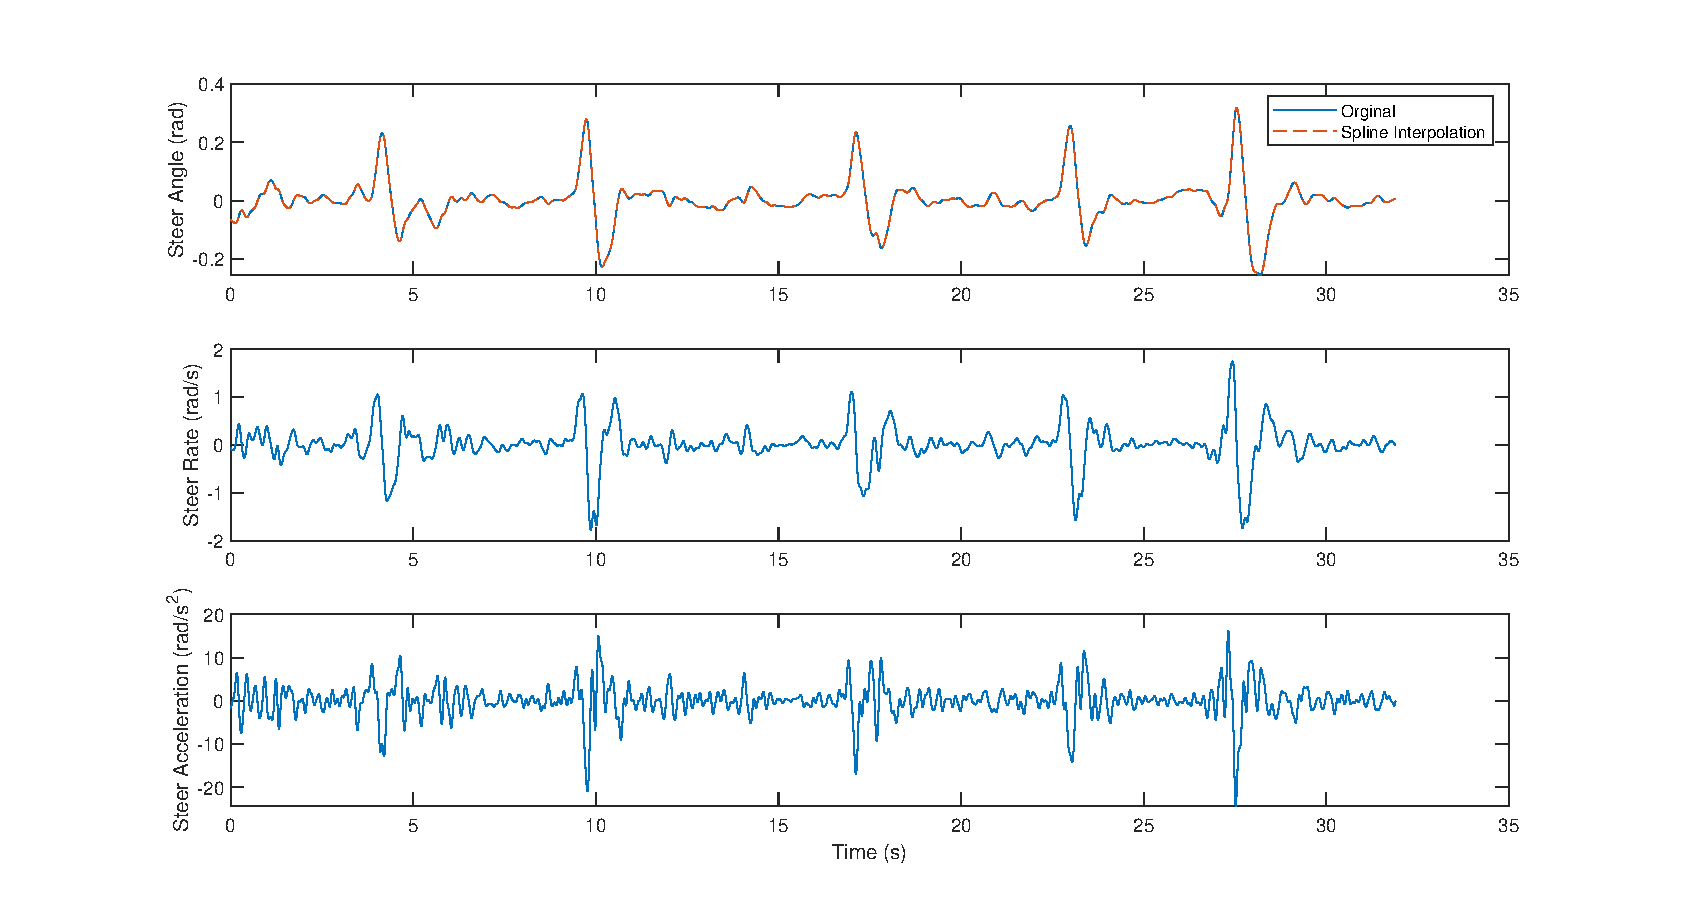
\includegraphics[scale=0.6]{images/steer_rates_spline.eps}
    \caption{Steering angle signal with its derivates produced by the piecewise cubic spline interpolation method.}
    \label{fig:spline}
\end{figure}
\section{Steering shaft moment of inertia and viscous friction}

In order to make estimation of applied rider torque, the damping coefficient and the inertia of the steering shaft needs to be determined. There are multiple ways to measure inertia of complex geometries. Here an estimation through a simple exprimental setup is chosen.

By connecting the steering shaft with two extension springs (see Fig.\ref{fig:figure1}) and measuring the oscillations of the steering angle \ensuremath{\delta}, a mechanical system is created where it it has to obey equation \ref{eq:1}.
\begin{equation}
    I_H\ddot{\delta}\left(t\right)+b_m\dot{\delta}\left(t\right)+2K\alpha^2\delta\left(t\right)=0
    \label{eq:1}
\end{equation}
where \ensuremath{K} the spring elastic constant and \ensuremath{\alpha} the moment arm shown in figure \ref{fig:figure1}. 
\begin{figure}[h]
\centering
\captionsetup{justification=centering,margin=2cm}
\includegraphics[scale=0.9]{images/figure1.png}
	\caption[Short title]{Spring-handlebar assembly  where \ensuremath{\alpha}  is the moment arm.}
\label{fig:figure1}
\end{figure}

 The springs ( \ensuremath{K=555 N/m} and slack length of \ensuremath{ 0.03m}) are attached to the handlebar and the system is perturbed. The measured steering angle signal from one of the perturbation tests is shown in figure \ref{fig:figure3}.The steering rate and acceleration signals are derived by the methods descirbed in section \ref{sec:rateAccel}. Equation \ref{eq:1} is then applied to all discrete time steps and so the system of equations \ref{eq:leastSquaresTORQUE} is created.
 \begin{equation}
     \begin{bmatrix}
         \ddot{\delta}_1 & \dot{\delta}_1   \\ \ddot{\delta}_2 & \dot{\delta}_2 \\ \vdots & \vdots \\ \ddot{\delta}_N & \dot{\delta}_N 
     \end{bmatrix} \begin{bmatrix}
         I_H \\ b_m
     \end{bmatrix} = -2K\alpha^2 \begin{bmatrix}
         \delta_1 \\ \vdots \\ \delta_N
     \end{bmatrix}
     \label{eq:leastSquaresTORQUE}
 \end{equation}
where \ensuremath{N} the length of the recorded signal.

Since equation \ref{eq:leastSquaresTORQUE} is linear in the parameters, the solution of the regression problem can be approximated by the use of the least squares method.
\begin{equation}
 \begin{bmatrix}
    I_H \\ b_m
\end{bmatrix} = -2K\alpha^2 \left(      \begin{bmatrix}
    \ddot{\delta}_1 & \dot{\delta}_1   \\ \ddot{\delta}_2 & \dot{\delta}_2 \\ \vdots & \vdots \\ \ddot{\delta}_N & \dot{\delta}_N 
\end{bmatrix} ^{T}       \begin{bmatrix}
    \ddot{\delta}_1 & \dot{\delta}_1   \\ \ddot{\delta}_2 & \dot{\delta}_2 \\ \vdots & \vdots \\ \ddot{\delta}_N & \dot{\delta}_N 
\end{bmatrix} \right)^{-1}      \begin{bmatrix}
    \ddot{\delta}_1 & \dot{\delta}_1   \\ \ddot{\delta}_2 & \dot{\delta}_2 \\ \vdots & \vdots \\ \ddot{\delta}_N & \dot{\delta}_N 
\end{bmatrix} ^{T}  \begin{bmatrix}
    \delta_1 \\ \ldots \\ \delta_N
\end{bmatrix}
\label{eq:leastSOLUTION}
\end{equation}
The system is perturbed 15 times so 15 sets of inertia and damping ratios are computed. The mean of the these was taken and  resulted in  \ensuremath{I_H = \mathbf{0.0960 \;kg\; m^2}} and   \ensuremath{b_m = \mathbf{0.2663\; N\; s^{-1}}}



\begin{figure}[h]
\centering
\captionsetup{justification=centering,margin=2cm}

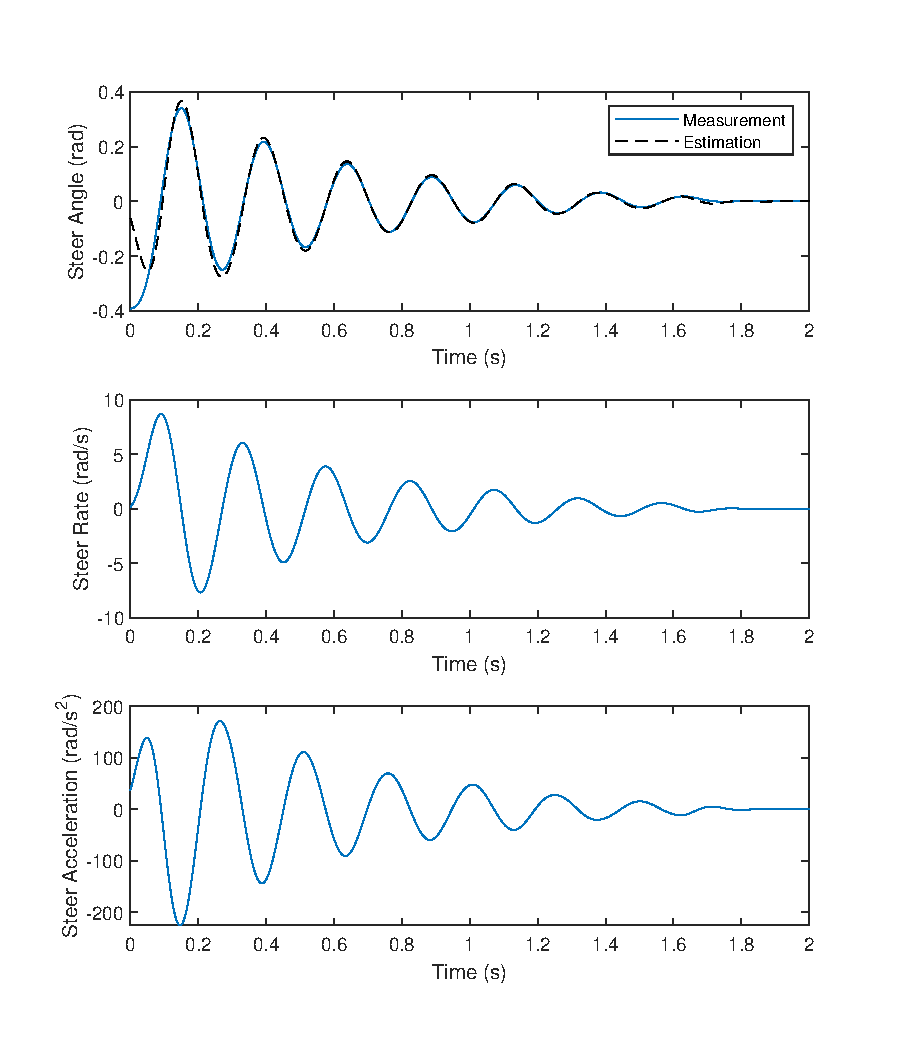
\includegraphics[scale=0.8]{images/figure3.eps}
	\caption[Short title]{Result of the first of fifteen oscillations. Blue lines indicate the  measured signals while the black dotted line is the output of the model given the values of inertia and damping estimated with the least squares method.}
\label{fig:figure3}
\end{figure}


% The damping coefficient is  \ensuremath{b=\mathbf{0.5845} \mathbit{Nms} }
\newpage
\section{Motor Torque Input Validation} \label{sec:torqueSensor}

\subsection{Design of torque sensor}
In order to validate that the torque exerted by the handlebar motor results in equivalent input rider torque  a torque sensor is designed and attached to the steering shaft. The most common torque sensor measurement principle uses bonded strain gauge technology, where the strain gauges are bonded to a suitably designed shaft.

In the torsion of a cylindrical shaft the strain is measured by the angle of twist or angular deflection. Unfortunately stain gauges can only detect compressive and tensile strain. The strain gauges are placed with such an orientation that the shearing stress is replaced by its equivalent principal stresses. The angle and the magnitude of the principal stresses are calculated by the use of the Mohr Circle. In this case the principal tension and compressive stresses are of the same magnitude as the shearing stress and are active at an angle of 45 degrees since it is  considered that no external compressive or tension force is present. 

In order to design a proper cylindrical shaft for the torque sensor the diameter of the shaft is chosen such that the strain measured in the strain gauges is within the detectable range (\ensuremath{\epsilon_{min}=10^{-5}} , \ensuremath{\epsilon_{max}=6\cdot10^{-4}}). For this application,  a hollow cylindrical shaft made of aluminum( \ensuremath{AL7075-O})is used so the unknowns are the inner and outer diameters. The strain is given in relation to the stress by Hooke’s law for isotropic materials by equation (\ref{eq:4}). The shearing stress is in turn given by equation (\ref{eq:5}). 


\begin{equation}
\epsilon=\frac{\sigma\cdot (1+\nu)}{E}
\label{eq:4}
\end{equation}

where \ensuremath{\nu} the Poisson's ratio and E the Young's Modulus (\ensuremath{Pa})
\begin{equation}
\tau=\frac{T\cdot r}{J}
\label{eq:5}
\end{equation}
where \ensuremath{J} is the polar moment of inertia (\ensuremath{m^4}), \ensuremath{r} the distance from center to stressed surface in the given position (\ensuremath{mm}), \ensuremath{T} the twisting moment (\ensuremath{Nm}).
 The polar moment of inertia of a circular hollow shaft can be expressed as
\begin{equation}
J = \frac{\pi \cdot (D^4 - d^4)} {32}                          
\label{eq:6}
\end{equation}
where \ensuremath{d} is shaft inside diameter (\ensuremath{mm}) and \ensuremath{D} is the shaft outside diameter (\ensuremath{mm}).

By inputing the above equations into a MATLAB script figure \ref{fig:figure4} was produced. The figure was created for a fixed inner diameter of \ensuremath{12 mm}, due to limitations in the machining process. It is evident that the lower the width of the shaft the higher detection of the low level torques. For this reason a width of 2 mm was chosen. This still means that  torques below \ensuremath{0.2 Nm } are not detectable. However the purpose of the torque sensor is not to provide acurate online measurements but to validate the input torques from the handlebar motor. The design of the resulting part is shown in \ref{fig:figure5}. 


\begin{figure}[h]
\centering
\captionsetup{justification=centering,margin=2cm}
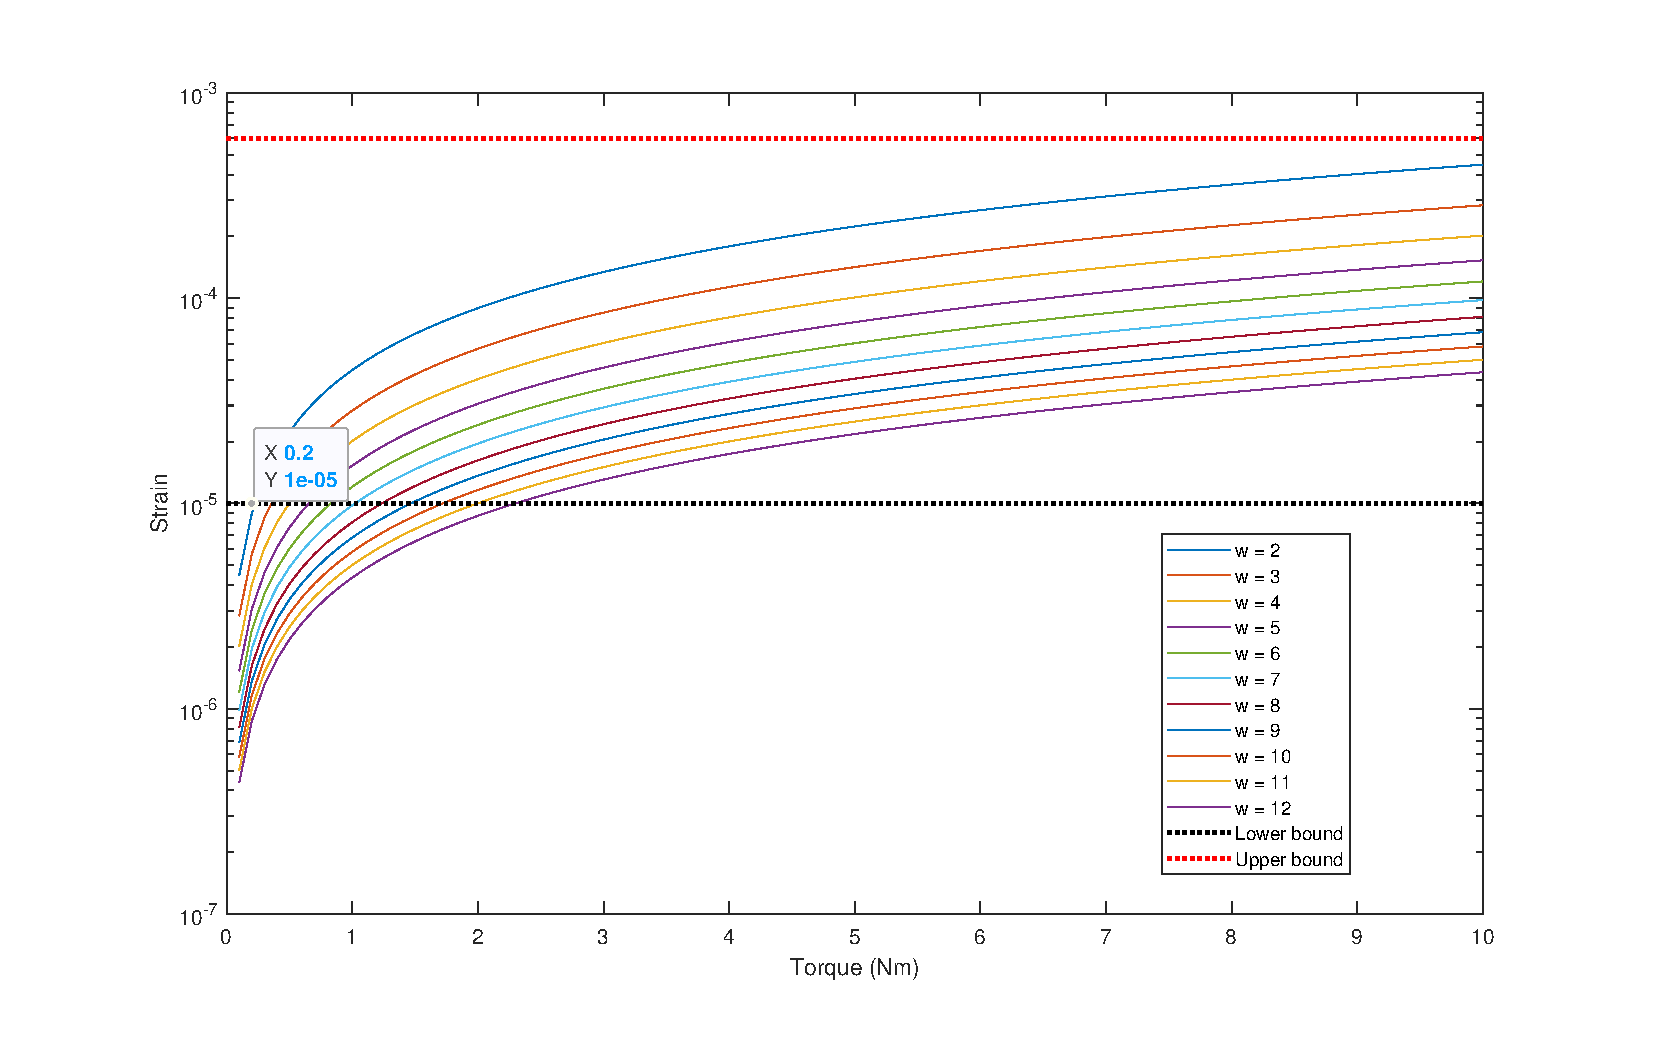
\includegraphics[scale=0.5]{images/figure4.eps}
	\caption[Short title]{Principal tensile strain in the 45 degree angle for various shaft widths (w).}
\label{fig:figure4}
\end{figure}


\begin{figure}[h]
\centering
\captionsetup{justification=centering,margin=2cm}

\includegraphics[scale=0.4]{images/sensor_schematic.png}
	\caption[Short title]{Schematic of the hollow shaft.}
\label{fig:figure5}
\end{figure}
\newpage
Because it is not an ideal hollow cylinder , the shearing stress  calculated analytically from the above equations needs to be validated. A static load simulation in SolidWorks is done to see how much different  is the shearing stress on the external surface. As it turns out the simulation showed a shearing stress similar to the one calculated by the equations. In \ref{fig:figure6} the simulation results for a loading of \ensuremath{10 Nm} is shown. For comparison the resulting shearing stress calculated analytically  is \ensuremath{10.0874\cdot 10^6 N/m^2 }. For proper measurements of  strain  the gauge  placement should gravitate towards the middle to avoid the spikes of shearing stress near the intersections between the main shaft and the cylindrical heads (see fig. \ref{fig:figure6})

\begin{figure}[h]
\centering
\captionsetup{justification=centering,margin=2cm}

\includegraphics[scale=0.6]{images/sensor_shear_SW.png}
	\caption[Short title]{Shearing stress for \ensuremath{10 Nm} loading in the axial direction.}
\label{fig:figure6}
\end{figure}

\subsection{Results}
In order to validate that the commanded torque in the handlebar motor is the same as the one actually applied in the handlebar, a trial identification run was conducted to simulate steer torque levels of the experiments. The signal of the input motor torque is compared with the output of the custom made torque sensor. The results are shown in figure \ref{fig:figure7}. The mismatch of the two signals for values lower than \ensuremath{0.5 Nm} is attributed to the fact that the sensor's strain gauges cannot accurately measure the strain in the material to produce realiable ouput as determined analytically beforehand. Also during the measurements a slight bias of the sensor was noted when  \ensuremath{0<\delta<\pi \char`\\
2}. Despite the aforementioned , the resulting Variance Accounted For (VAF) was equal to \ensuremath{90.77 \%} and was deemed that the motor command torque  is indeed what is beeing applied in the steering shaft so in all subsequent calculation it was taken as ground truth.

\begin{figure}[h]
    \centering
    \captionsetup{justification=centering,margin=2cm}

    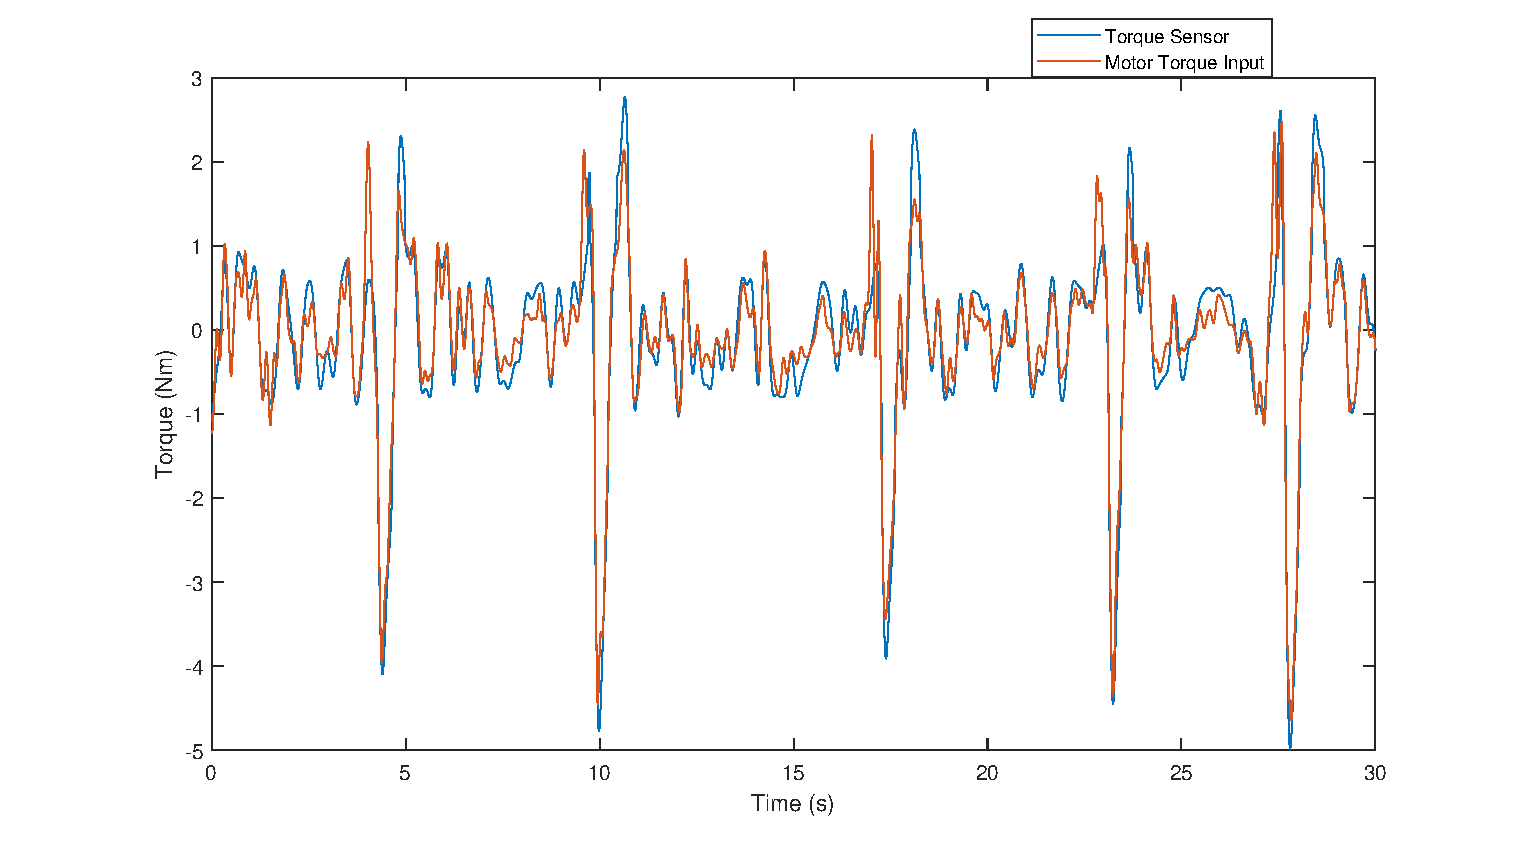
\includegraphics[scale=0.5]{images/results_torque_sensor.eps}
        \caption[Short title]{Measurement of torque sensor compared to the commanded torque of the handlebar motor.}
    \label{fig:figure7}
\end{figure}